% Notes on the writing of the Master Thesis
% Book: How to Write a Lot, Paul Silvia, 2nd Edition
% Book: Getting Things Done, David Allen
%
%
% Mögliche Abgrenzung von anderen: Den hybriden Ansatz von SBST mit DSE verwenden, 
% so wie im Paper von Baars et al.
%
% Mögliche weitere Evaluation: Vergleiche die Coverage von generierten Tests zu der 
% Coverage von manuell geschriebenen Tests von Entwicklern in evaluierten Programmen.
% 

\documentclass{article}
% Please do not change this options...
\usepackage[a4paper, total={6in, 10in}]{geometry}
\usepackage{graphicx}
\graphicspath{ {./img/} }
\usepackage{todonotes}
\usepackage{acronym}
\usepackage[T1]{fontenc}
\makeatletter
\newcommand\BeraMonottfamily{%
  \def\fvm@Scale{0.85}% scales the font down
  \fontfamily{fvm}\selectfont% selects the Bera Mono font
}
\makeatother


\usepackage{listings}
\lstset{
  numbers=left,
  xleftmargin=2.5em,
  framexleftmargin=2.5em,
  frame=tb,
  stepnumber=1,    
  firstnumber=1,
  numberfirstline=true,
  basicstyle=\BeraMonottfamily,
  identifierstyle=,
  stringstyle=\ttfamily,
  %keywordstyle=\color{OliveGreen},
  keywordstyle=,
  showstringspaces=false
}

% This package must be declared last
\usepackage{cleveref}

\begin{document}

\title{Master Thesis}
\author{Vsevolod Tymofyeyev}
\date{\today}
\maketitle

\tableofcontents
\section{Introduction}
In der Programiersprachenwelt, in der es zwei große Fronten gibt (low-level Sprachen, die auf Kosten von Sicherheit mehr Performanz bieten und high-level Sprachen, die durch bestimmte Konstrukte wie Garbage-Collector Sicherheiten für Programmierer bieten, die jedoch zu Laufzeit-Overhead führen) versucht Rust beides zu verbinden. Die Sprache für Systemprogrammierung verspricht eine ähnlich hohe Performanz wie C++ mit erweiterter Typ- und Speichersicherheit. Invarianten werden zur Kompilierzeit sichergestellt, wodurch Abstraktionen mit keinen Laufzeitkosten verbunden sind (sogenannte Zero-Cost-Abstractions). Diese Symbiose führte dazu, dass die Sprache besonders attraktiv auf Entwickler wirkte, wodurch sie trotz ihres sehr jungen Geschichte bereits seit mehreren Jahren die Beliebtheitsrankings stürmt~\cite{StackOverflow2020}. Selbst Spitzenkonzerne erwägen eine Nutzung oder gar Umschreibung von Teilen ihrer Codebase nach Rust. Laut Microsoft und Google sind 70\% der in ihrer Software in den vergangenen Jahren gefundenen Fehler auf Speicherlecks zurückzuführen, hervorgerufen durch die weitverwendeten unsicheren Sprachen wie C und C++~\cite{Microsoft2019MemoryBugs, RustInAndroid}. Microsoft, SpaceX, Google, Amazon AWS und viele andere Unternehmen fingen bereits an, Rust in ihren Produkten zur erhöhten Sicherheit zu verwenden~\cite{MicrosoftJoinsRust, AmazonLovesRust, RustInAndroid, GoogleRustFoundation}. 

\todo{Ein sanfter Wechsel zur Testgenerierung wäre angebracht.} Software muss getestet werden, um möglichst früh Fehler zu finden, bevor das Produkt beim Endnutzer landet. Allerdings ist das Schreiben der Tests oft langwierig, kostet viel Zeit und mögliche Ausführungsfälle können von Testern vor allem in sehr komplexen Programmen übersehen werden. Aus diesem Grund beschäftigt sich die Forschung seit Jahren mit der Automatisierung dises Prozesses. 

\section{Background}
\subsection{Test Generation in General}
\todo{Structural, functional, etc. testing}
Testsgenerierung ist ein aktiv erforschtes Feld in der Wissenschaft. Im Idealfall kann für ein Programm eine Testsuite von Unit Tests generiert werden, die alle möglichen Pfade im \ac{SUT} abdecken und gleichzeitig die Korrektheit der Ausführung jedes einzelnen Pfades durch automatische Orakel überprüft, beispielsweise durch Assertions. Ein Orakel ist ein Mechanismus zum Überprüfen, ob ein Output bei einem gegebenen Input richtig ist, beispielsweise mit Hilfe einer formalen Spezifikation~\cite{10.1145/1569901.1570127}. Leider ist das oft nicht möglich. Zum einen können in einem Programm Ausführungspfade existieren, die schlicht unter keinen Umständen erreicht werden können. Zum anderen hat Software nur sehr selten eine formale Spezifikation, die bei der Generierung verwendet werden kann, um Orakel zu generieren. Somit muss in den meisten Fällen ein Entwickler bzw. Tester die generierte Testsuite manuell mit Orakeln versehen (dazu muss er/sie natürlich selbst wissen was das richtige Verhalten ist)~\cite{Fraser_2013}. Dazu muss die generierte Testsuite aber auch möglichst klein und für den Menschen verständlich gehalten werden. 

Bei einer Testgenerierung wird das Coverage-Kriterium oft als eine Leitlinie benutzt~\cite{Fraser_2011}. Ein Coverage-Kriterium ist eine Sammlung von Test-Zielen, die typischerweise eins nach dem anderen abgearbeitet bzw. abgedeckt werden, wobei die notwendigen Input-Daten beispielsweise symbolisch oder such-basiert ermittelt werden. Eine beliebte Art des Coverage-Kriteriums ist die Branch-Coverage. 

Branches sind z. B. Arme einer if-Verzweigung oder eines Schleifenkopfes. Diese werden dann ausgeführt, wenn ein bestimmter boolischer Ausdruck zu \lstinline{true} bzw. \lstinline{false} evaluiert. Branches können auch verschachtelt sein, und um passende Werte zu finden, um einen (verschachtelten) Branch zu erreichen, kann symbolic execution bzw. seine dynamische Erweiterung mit konkreten Werten verwendet werden. Dabei wird ein Pfad aufgebaut, der mit einem \ac{SMT}-Solver nach konkreten Werten (falls solche existieren und der Pfad überhaupt erreichbar ist) aufgelöst werden kann. Eine Alternative zur symbolic Execution ist eine meta-heuristische Suche. Fraser und Arcuri~\cite{Fraser_2011} listen ein paar verwante Paper dazu auf. 

\subsection{Automatically Generated Oracles}
\label{sec:generated-oracles}
Davis and Weyuker~\cite{10.1145/800175.809889} haben den Begriff non-testable programs einfegührt, der solche Programme einschließt, für die es keinen Testorakel gibt oder ein Testorakel praktisch nicht umsetzbar ist, und man somit das Ergebnis der Berechnung nicht auf Korrektheit überprüfen kann. Dazu gehören Programme, die entweder erstellt wurden, um das Ergbenis überhaupt zu erfahren, oder Programme, die zu viele Ergebnisse liefern, um sie alle zu überprüfen, oder der Entwickler hatte die Spezifikation missverstanden. Um das Problem eines fehlenden Orakels zu lösen, führten die Autoren einen sogenannten Pseudoorakel ein. Ein Pseudoorakel ist ein zweites, unabhängig implementiertes Programm, das derselben Spezifikation entsprechen muss. Es ist wichtig, dass die zwei Programme von separaten Teams ohne Zwischenkommunikation erstellt werden, damit keine Missverständnisse von einem in das andere Team propagieren können. Anschließend können die Ergebnisse der Berechnungen des originalen Programms und des Pseudoorakels verglichen und es kann über die Validität entschieden werden. 

Das manuelle Erstellen von Pseudoorakeln ist sehr mühselig und ist im Kontext von Testgenerierung für große Projekte nicht lohnenswert. Harman et al.~\cite{1265732} haben das Prinzip der Testability Transformations vorgestellt. Diese sind Quelltext-zu-Quelltext Transformationen, die zum Verbessern der Performanz verschiedener Testgenerierungstechniken führen sollen. McMinn~\cite{10.1145/1569901.1570127} hat diese Idee aufgegriffen und vorgeschlagen, Pseudoorakel für ein gegebenes Programm automatish zu generieren. Er wendet Testability Transformations an, um das originale Programm zu verändern und eine zweite Version zu generieren, die scheinbar gleiche Ausgaben wie die originale haben sollte, es jedoch zu Diskrepanzen kommen kann. Dazu hat er zwei Beispiele aufgeführt: Fließkomma-Arithmetik und Multithreading in Java. Beim Ersteren werden, beispielsweise Additionen zwischen primitiven Fließkommatypen, die nach dem IEEE-Standard etwas ungenau in den hinteren Nachkommastellen sind~\cite{10.1145/103162.103163}, durch Javas BigDecimal vertauscht. Zum Beispiel führt die Berechnung~$0.1 + 0.1 + 0.1$ in Java zum Ergebnis~$0.30000000000000004$, anstatt~$0.3$ (siehe~\cref{lst:java-transformations}).

\begin{lstlisting}[language=Java, caption=Comparing floating-point arithmetic in Java using double compared to BigDecimal~\cite{10.1145/1569901.1570127}, label=lst:java-transformations]
System.out.println(0.1 + 0.1 + 0.1);
// Ausgabe: 0.30000000000000004

System.out.println(
    new BigDecimal("0.1").add(
        new BigDecimal("0.1").add(
            new BigDecimal("0.1")
        )
    )
);
// Ausgabe: 0.3
\end{lstlisting}
In einem anderen Beispiel wendet McMinn Transformationen zum Serialisieren/Deserialisieren eines Multithreading-Programm. Dabei werden Methoden einer Klasse mit Javas \lstinline{synchronize} versehen bzw. das Schlüsselwort wird bei bereits synchronisierten Methoden entfernt. \lstinline{synchronize} sorgt dafür, dass nur ein Thread gleichzeitig die jeweilige Methode verwenden darf. In der Evaluation versucht der Autor, die durch Transformationen generierten Orakel mit Hilfe für eine genetisch-basierte Suche nach Input-Daten zu verwenden, die die Diskrepanz zwischen den Ausgaben eines originalen Programms und seines Psudoorakels maximieren. Damit können nicht nur potenzielle Bugs automatisch entdeckt (Diskrepanz), sondern auch ihr Schweregrad gemessen (Größe der Diskrepanz) werden. Die Idee von automataisch generierten Pseudoorakel wurde auch von Fraser und Arkuri~\cite{Fraser_2013} aufgegriffen. \todo{Da fehlt was}

\subsection{Random Testing}
\subsection{Search-based Techniques}
Der potenzielle Suchraum für mögliche Inputdaten selbst bei einem sehr simplen Programm kann unendlich groß sein. Metaheuristische Ansätze versprechen eine Abhilfe. Das sind keine geschlossenen Algorithmen an sich, sondern Strategien, die auf spezifische Probleme angepasst werden können. Für die Generierung von Testdaten wird eine problem-spezifische Fitnessfunktion definiert, mit deren Hilfe die Qualität möglicher Lösungen des Problems verglichen werden kann~\cite{McMinn_2004}. Metaheurische Suche wird nicht nur für Testdatengenerierung verwendet. Andere Verwendungen umfassen:
\begin{itemize}
	\item Coverage der Programmstruktur als Teil einer White-Box Teststrategie,
	\item das Auswerten eines spezifischen Programmfeatures nach seiner formalen Spezifikation,
	\item Versuche, automatisch Fehlerbedingungen oder Brüche von Assertions in einem Programm herbeizurufen
	\item Verifizierung nicht-funktionaler Features, beispielsweise worst-case Ausführungszeit eines Programmteils finden.
\end{itemize}
\subsubsection{Genetic Algorithms}
McMinn hat ein super Beschreibung von genetischen und evolutionären Algorithmen, Selektion, Crossover, Mutation, fortgeschrittene Repräsentationen von Individuen~\cite{McMinn_2004}.

In seinem Paper beschreibt Harman~\cite{Harman}, wie bestimmte Variablen innerhalb von Verzweigungsknoten bei der Suche rausgefiltert werden können, weil sie keinen Einfluss auf die Branch Distance haben. Somit wird der Suchraum verkleinert. 

\subsubsection{Many-objective Search}
 Fraser und Arcuri~\cite{Fraser_2013} haben einen neuen Ansatz für die Generierung von Tests basierend auf der Branch-Abdeckung vorgeschlagen, names Whole Test Suite Generation. Frühere Ansätze steuern jeweils ein Coverage Objective an und implizieren, dass alle Objectives unabhängig, gleich schwer zu erreichen sind und überhaupt erreichbar sind. Jedoch sind Objectives, also in dem Fall Branch Coverage Goals, in einem Programm oft von einander abhängig. Viele Branches erfordern, dass andere Branches zuvor in der Ausführung gedeckt werden. Es können auch Fälle eintreten, in denen einige Objectives überhaupt nicht erreichbar sind~\cite{Goldberg_1994}. Außerdem können in einer Ausführung gleich mehrere Objectives gedeckt werden (eine sogenannte kollaterale Abdeckung)~\cite{Fraser_2011}. Aus diesem Grund stellen die Autoren einen anderen Ansatz, bei dem versucht wird, durch generierte Tests alle Branch Goals auf einmal abzudecken. 

Fraser und Arcuri~\cite{Fraser_2011} improve over the state of the art in search-based testing by (1) handling dependencies among predicates, (2) handling test case length dynamically without applying exploration imped- ing constraints, and (3) giving guidance towards reaching test goals in private functions. In their work, the authors target difficult problems, which automatic test oracles cannot be generated for, as described in~\cref{sec:generated-oracles}, as opposed to~\cite{Pacheco_2007, Godefroid_2005} \todo{Auf die beiden Tools eingehen und etwas dazu erzählen, wahrscheinlich aber im Abschnitt State of the Art}. In their approach, they try to maximize the branch coverage of the generated test suites with the smallest possible tests, so that a developer can add oracles to the generated tests manually with low congnitive load (the generated tests should be easily understandable).

Der MOSA Algorithmus, auch als Many-Objective Sorting Algorithm~\cite{Panichella_2015} bekannt, ist ein mehr oder weniger innovativer Algorithmus, der unter anderem auch auf die Entwicklung von Fraser und Arcuri~\cite{Fraser_2013} setzt. 
\subsection{Dynamic Symbolic Execution}


\section{State of the Art}
\subsection{Fuzzer for Rust}
\subsection{Test Generators for Rust}

\section{Search-based Unit Test Generation in Rust}
\begin{figure}[h]
\caption{Übersicht des Testify Tools}
\centering
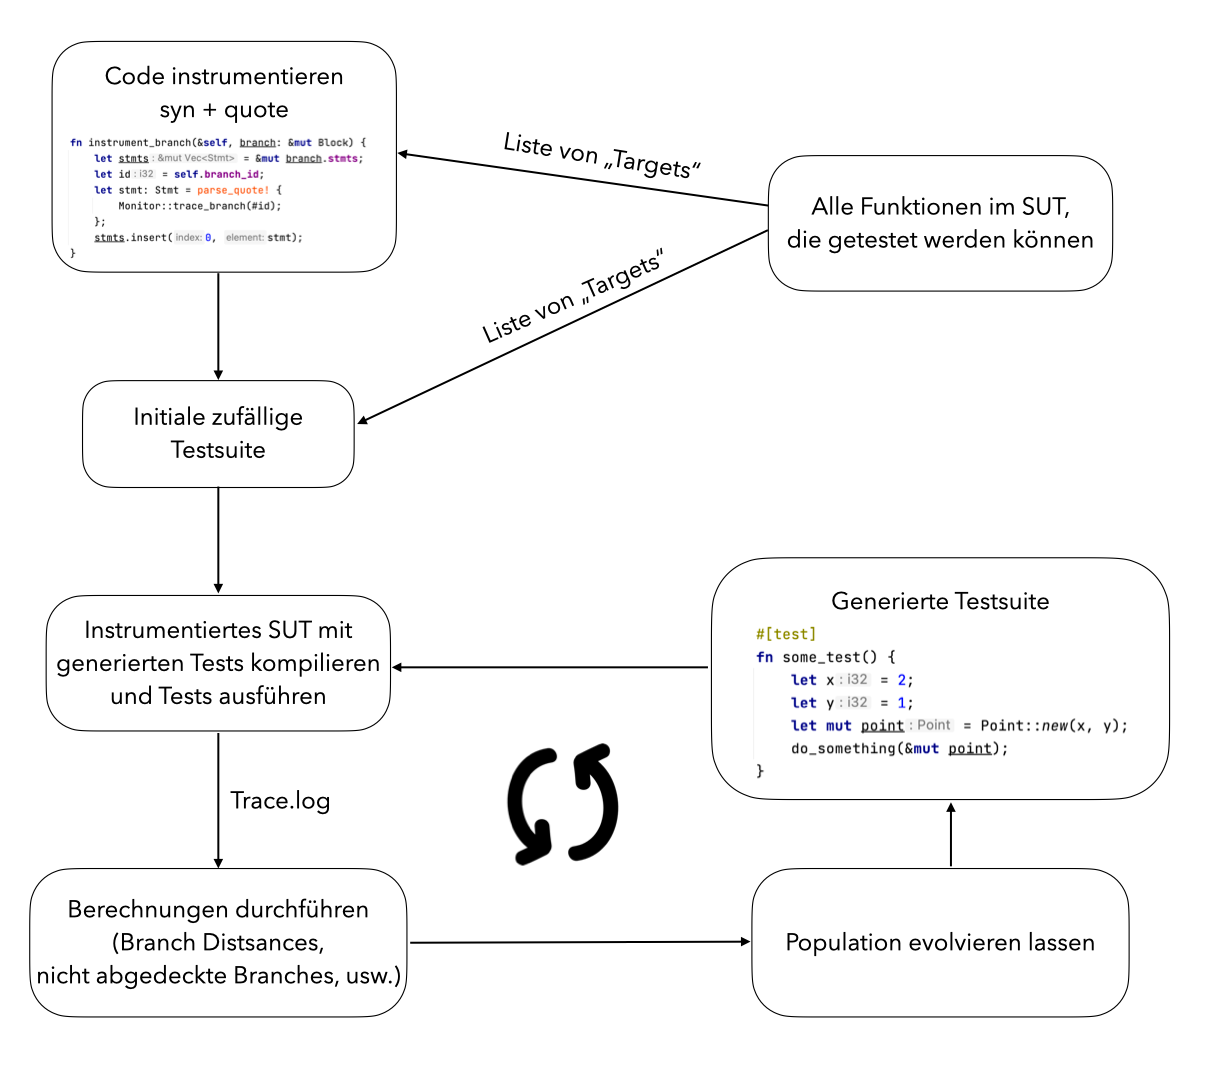
\includegraphics[width=\textwidth]{testify-overview}
\label{fig:testify-overview}
\end{figure}
\subsection{Testability Transformations}
\subsection{Instrumentation}
\subsection{Test Suite Optimization}
Figure~\cref{fig:testify-overview} illustrates the main steps in the Testify Tool: It starts by instrumenting the \ac{SUT} and inserting necessary statements to trace a programm execution. Then, a random test suite is generated based on the \ac{SUT} and evolved using evolutionary search towards a specified fitness goal. At the end, the test suite with the highest coverage is returned. 

\subsubsection{Problem representation}
Hier wird die Repräsentation einer Lösung bzw. eines Individuums beschrieben. Laut McMinn~\cite{McMinn_2004} sollte eine Enkodierung der Lösung so gewählt sein, dass ähnliche Lösungen ebenfalls \"Nachbarn\" im repräsentierten Suchraum sind. Dadurch kann die Suche leicht von einer zur ähnlichen Lösung durch einfache Modifikationen der Repräsentation fortgeführt werden. Fraser und Arcuri schlagen folgendes zu Repräsentation der Lösung vor~\cite{Fraser_2011}: Eine Lösung ist hier eine Test Suite~$T$, die im Grunde ein Set von Unit Tests ist und für welchen gilt: Wenn~$|T| = n$, dann~$T = \{t_1, t_2, ... ,t_n\}$. 

Ein Unit Test ist demnach eine Liste von Statements, die Teile des \ac{SUT} ausführen, um ein gewisses Objective (bzw. Branch) zu erreichen und abzudecken. Jedes Statement ist ein Wert~$v(s_i)$, welcher von einem der fünf folgenden Typen~$\tau(v(s_i))$ sein kann:
\begin{itemize} 
	\item \textbf{Primitive Statements} repräsentieren numerische Variablen, z. B. \lstinline{let v = 42}. Der Wert und Typ des Statements werden von der primitiven Variable bestimmt. 
	\item \textbf{Konstruktor-Statements} generieren neue Instanzen eines gegebenen Structs, z. B. \lstinline{let s = SomeStruct::new()}. Der Wert und Typ des Statements werden vom Struct bestimmt. Ein Konstruktor kann Parameter haben, denen ebenso der Wert aus dem Set~$\{v(s_k) | 0 \leq k < i\}$ zugewiesen wird.
	\item \textbf{Attribut-Statements} greifen auf die public member variables von Objekten, z. B. \lstinline{let b = a.x}. Der Wert und Typ eines Attribut-Statements sind von der member variable abhängig. Die Quelle der member variable, also~\lstinline{a}, muss ebenso Teil des Sets~$\{v(s_k) | 0 \leq k < i\}$ sein. 
	\item \textbf{Methoden-Statements} führen Methoden auf Objekten aus oder rufen statische Methoden auf, z. B. \lstinline{let b = a.len()}. Hier wieder, das Quellobjekt und jegliche Parameter der Methode müssen Teil des Sets~$\{v(s_k) | 0 \leq k < i\}$ sein. Der Wert und Typ des Statements werden vom Return-Wert der Methode bestimmt. 
	\item \textbf{Funktionen-Statements} führen lose bzw. frei stehende Funktionen aus, z. B. \lstinline{let a = do_something()}. Die möglichen Parameter einer solchen Funktion müssen Teil des Sets~$\{v(s_k) | 0 \leq k < i\}$ sein. Der Wert und Typ des Statements werden vom Return-Wert der Funktion bestimmt. 
\end{itemize}

Die Sammlung von verfügbaren Structs, deren Konstruktoren, Methoden, Felder und frei stehende Funktionen sind ein sogenannter Test Cluster~\cite{Fraser_2011}. Die Größe einer Test Suite sowie einzelner Tests ist dabei dynamisch und kann sich (fast) beliebig verändern. Da für die meisten generierten Tests keine Testorakel zur Verfügung stehen werden, soll die Größe der Test Suite sowie der einzelnen Tests eine Obergrenze haben (kein Mensch möchte tausende Zeilen lange Tests durchlesen, um am Ende eine passende Assertion zu überlegen).

\subsubsection{Fitness Function}
Eine gute Fitnessfunktion ist sehr wichtig bei der Suche nach Lösungen. Lösungen, die in einer bestimmten Weise \"besser\" als andere sind, sollen mit besseren Fitnesswerten belohnt werden. Was auch immer eine bessere Fitness ist, eine höhere oder niedrigere Fitness hängt davon ab, ob die Suchstrategie versucht, die Fitnessfunktion zu maximieren oder zu minimieren~\cite{McMinn_2004}. Dieser Ansatz wird sich voraussichtlich auf Branch Coverage konzentieren. EvoSuite instrumentiert in der originalen Implementierung Java SUT auf Bytecode-Level und im Bytecode werden alle Loops usw. in die einfachen if-Verzweigungen überführt. Das Ziel ist es, die optimale Lösung zu finden, d. h. eine Test Suite, die möglichst hohe Branch-Coverage hat. Gleichzeitig soll es aber keine andere Testsuite geben, die bei gleicher Branch-Coverage kleiner ist bzw. kleinere Tests enthält. Einige Branches, sogenannte infeasible Branches, können evtl. gar nicht abgedeckt werden, entweder aufgrund der limitierten Repräsentation der Lösung oder weil es keine passenden Inputs existieren. Somit werden solche Tests bevorzugt bei der Evolvierung bevorzugt, die eine höhere Fitness bzgl. der Branch-Coverage haben. Bei zwei Tests mit der gleichen Coverage wird der kürzere bevorzugt. 

Um die Suche voranzutreiben, können verschiedene Heuristiken verwendet werden. \todo{Welche gibt es überhaupt?} Eine der weitverbreitesten ist Branch Distance. McMinn~\cite{McMinn_2004} beschreibt eine Sammlung von Regeln, die rekursiv angewendet werden können, um Distanz bei allen möglichen Prädikaten zu berechnen. Wenn die Ausführung des \ac{SUT} bei gegebenen Inputdaten in einem bestimmten Branch landet, so kann eine lokale Suche angewendet werden. Es wird mit Hilfe einer lokalen Fitnessfunktion abgeleitet, wie nah das Prädikat zum Auswerten zu \lstinline{true} ist. Zum Beispiel, bei einem Prädikat~\lstinline{x >= 10} und~\lstinline{x = 5} (während der Ausführung) wird der \lstinline{false} Branch getroffen. Die Distanz zum \lstinline{true} Branch beträge somit~$10 - 5 + k$ mit~$k \geq 1$. Dabei wird jedes Prädikat im \ac{SUT} instrumentiert, um die Distanzen zu anderen Branches während der Ausführung des \ac{SUT} zu tracen. Die Branch-Distanz muss noch normalisiert werden (je nach Werten kann es schnell zu Extremen kommen). Arcuri~\cite{Arcuri_2011} beschreibt in seiner Arbeit, welchen Einfluss die Normalisierung der Branch-Distanz auf die Effektivität einer such-basierten Testgenerierung hat. 


\subsubsection{Bloat Control}
Hier wird beschrieben, wie man verhindern kann, dass die Größe der Test Suite und einzelner Tests ausartet. Fraser und Arcuri~\cite{Fraser_2011} haben ein paar Gedanken dazu. 

\subsubsection{Search Operators}
Suchoperatoren wie Crossover, Mutation und Random Test Case werden hier beschrieben. Natürlich haben auch Fraser und Arcuri~\cite{Fraser_2011} eine ausführliche Beschreibung der Funktionsweise. 

\section{Evaluation}
\subsection{Setup}
\subsection{Threats to Validity}
\subsection{Code Coverage Comparison with Manually Written Tests}
\subsection{Code Coverage Comparison with Other Tools}


\section{Conclusion}

\section{Future Work}

\appendix
\chapter{Acronyms}
\begin{acronym}
	\acro{SUT}{System Under Test}
	\acro{CUT}{Class Under Test}
	\acro{MUT}{Method Under Test}
	\acro{SMT}{Satisfiability Modulo Theories}
	\acro{GA}{Genetic Algorithm}
	\acro{EA}{Evolutionary Algorithm}
	\acro{MOSA}{Many-Objective Sorting Algorithm}
	\acro{DynaMOSA}{Many-Objective Sorting Algorithm with Dynamic target selection}
	\acro{WS}{Whole Suite}
	\acro{WSA}{Whole Suite with Archive}
	\acro{SBST}{Search-based Software Testing}
	\acro{SBSE}{Search-based Software Engineering}
	\acro{ATP}{Automated Theorem Prover}
	\acro{DSE}{Dynamic Symbolic Execution}
	\acro{IR}{Intermediate Representation}
	\acro{MOA}{Multi- and Many-Objective Algorithm}
	\acro{DDG}{Data Dependence Graph}
	\acro{HIR}{High-level Intermediate Representation}
	\acro{THIR}{Typed HIR}
	\acro{MIR}{Mid-level Intermediate Representation}
	\acro{AST}{Abstract Syntax Tree}
	\acro{CFG}{Control Flow Graph}
	\acro{CDG}{Control Dependence Graph}
	\acro{API}{Application Programming Interface}
	\acro{NSGA-II}{Non-dominated Sorting Genetic Algorithm II}
	\acro{TCP}{Transmission Control Protocol}
	\acro{SSA}{Static Single Assignment}
\end{acronym}


\bibliographystyle{unsrt}
\bibliography{bibliography}
%\nocite*{}
\end{document}